%!TEX encoding = UTF-8~Unicode
%!TEX program = pdflatex
%!BIB program = biber

\documentclass[11pt,a4paper,twoside]{report}
\usepackage[a4paper, top=25mm, bottom=25mm, inner=30mm, outer=30mm, twoside]{geometry}

\usepackage[polish]{babel}
\usepackage[T1]{fontenc}
\usepackage[utf8]{inputenc}
\usepackage{lmodern}
\usepackage{amsmath}
\usepackage{url}
\usepackage{fancyhdr}
\usepackage{footnote}
\usepackage{float}
\usepackage{pdfpages}
\usepackage{multirow}
\usepackage{makecell}

\usepackage{listings}

\usepackage[algochapter,boxed,lined,linesnumbered]{algorithm2e}
\renewcommand{\algorithmcfname}{Algorytm}

\usepackage{xcolor}
\usepackage{url}
\usepackage{icomma}
\usepackage{microtype}

\usepackage[unicode,bookmarksopen,bookmarksnumbered]{hyperref}
\usepackage{titlepic}
\usepackage{graphicx}
\usepackage{subcaption}
\usepackage{array}
\usepackage[font=footnotesize,format=hang,labelfont=bf]{caption}

\usepackage{indentfirst}
\newcommand{\HRule}[1]{\rule{\linewidth}{#1}}

\fancyhf{}
\renewcommand{\headrulewidth}{0pt}
\pagestyle{fancy}
\fancyfoot[LE,RO]{\thepage}

\usepackage{csquotes}

\clubpenalty=10000
\widowpenalty=10000

\begin{document}
%-------------------------------------------------------------------------------
\title{ \textsc{Przetwarzanie cyfrowe obrazów} \\ [1.0cm]
		\LARGE \textbf{System do rozpoznawania loga Pepsi} \\ [1.0cm]
		\normalsize \today}
\date{}
\author{Adam Kowalewski}
\titlepic{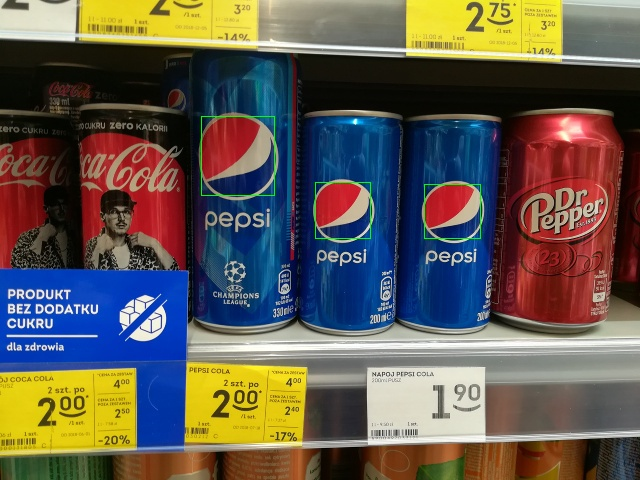
\includegraphics[width=0.8\textwidth]{img/pepsi0.png}}
\maketitle
%-------------------------------------------------------------------------------

\section*{1. Wstęp}

	Niniejsza dokumentacja opisuje system służący do rozpoznawania loga napoju Pepsi na zdjęciach cyfrowych. Napisany on został jako aplikacja konsolowa z wykorzystaniem języka C++17. Rozpoznawanie loga Pepsi wykonywane jest w oparciu o klasyczne metody przetwarzania obrazów, tj. poprzez segmentację kolorów oraz klasyfikację w oparciu o niezmienniki momentowe. Mimo, iż aplikacja zbudowana została w oparciu o bibliotekę OpenCV, wszelkie algorytmy służące przetwarzaniu obrazów zostały zaimplementowane samodzielnie. Program oferuje przystępny interfejs konsolowy oraz możliwość konfiguracji parametrów algorytmów przy pomocy plików JSON. Oprócz zestawu zdjęć przykładowych, dla których można zweryfikować działanie programu, dostarczony został obszerny zestaw testów jednostkowych, testujących wybrane moduły programu.

\section*{2. Korzystanie z programu}

	\subsection*{2.1. Wykorzystane technologie}

		Aplikacja została napisana z użyciem języka C++17. System budowania oparty został o program \texttt{CMake}, w wersji 3.10.2. Aplikacja została przetestowana z kompilatorem \texttt{GCC}, w wersji 8.3.0. Jako menadżera pakietów wybrano system \texttt{Conan} w wersji 1.10.1. Aplikacja korzysta z następujących bibliotek:
		\begin{itemize}
			\item \texttt{OpenCV} - Jedynie podstawowe struktury, takie jak \texttt{cv::Mat}, \texttt{cv::Size}, \texttt{cv::Point}, \texttt{cv::Vec}. Wszelkie algorytmy przetwarzające obrazy zostały napisane samodzielnie
			\item \texttt{CLIUtils::CLI11} - Autorstwa Henry'ego Schreinera. Ułatwia tworzenie interpretera linii poleceń w aplikacji konsolowej.
			\item \texttt{nlohmann::json} - Autorstwa Nielsa Lohmanna. Z jej użyciem zrealizowano wczytywanie konfiguracji z plików JSON
			\item \texttt{catchorg::Catch2} - Ułatwia pisanie testów jednostkowych z wykorzystaniem technik TDD, BDD
			\item \texttt{gabime::spdlog} - Autorstwa Gabi Melman. Ułatwia generowanie komunikatów diagnostycznych
		\end{itemize}

	\subsection*{2.2. Budowanie}

		Do zbudowania aplikacji wymagane jest posiadanie globalnie zainstalowanej biblioteki OpenCV. Poniższe kroki opisują sposób kompilacji w systemie Linux:
		\begin{verbatim}
		    > git clone https://github.com/akowalew/pepsi-logo-detector
		    > cd pepsi-logo-detector && mkdir build && cd build
		    > conan install .. -s compiler=gcc -s compiler.version=8
		    > export CXX=g++-8 && cmake .. -DCMAKE_BUILD_TYPE=Debug
		    > make -j5
		\end{verbatim}

		Po zbudowaniu aplikacji użytkownik ma do dyspozycji dwa foldery: \texttt{bin} oraz dowiązany \texttt{assets}. W pierwszym znajdują się pliki wykonalne, zaś w drugim przykładowe obrazy, na których można przetestować algorytm.

	\subsection*{2.3. Uruchamianie}

		Do wykrywania loga pepsi służy program \texttt{find\_logos}. Jako pierwszy parametr przyjmuje ścieżkę do obrazka wejściowego, natomiast drugi, opcjonalny, wskazuje ścieżkę do obrazka wynikowego. Jeśli go pominiemy, wynik algorytmu zostanie przedstawiony na ekranie. Dodatkowo, flaga \texttt{-v} (\texttt{--verbose}) spowoduje wygenerowanie komunikatów diagnostycznych oraz wyświetlenie wszystkich zdjęć pośrednich w trakcie przetwarzania przez algorytm. Przykładowe wywołanie programu:

		\begin{verbatim}
		    > ./bin/find_logos assets/camera/0 -v
		\end{verbatim}

		Do dyspozycji użytkownika przygotowano dwa zestawy zdjęć testowych: pochodzących z kamery smartfonu oraz z internetu (odpowiednio nazwane katalogi \texttt{camera} oraz \texttt{net}).

		Użytkownik może modyfikować parametry działania algorytmu detekcji poprzez ich zmianę w pliku \texttt{config.json}. Poniżej przedstawiono przykładową konfigurację potoku przetwarzania:

		\begin{verbatim}
		{
		    "blue_range": { "min": [100, 75, 0], "max": [130, 255, 255] },
		    "blue_blob_area_range": { "min": 200, "max": 2500 },
		    "blue_blob_hu0_range": { "min": 0.30, "max": 0.50 },
		    "blue_blob_hu1_range": { "min": 0.05, "max": 0.15 },

		    "red_range": { "min": [165, 75, 75], "max": [10, 255, 255] },
		    "red_blob_area_range": { "min": 500, "max": 3000 },
		    "red_blob_hu0_range": { "min": 0.18, "max": 0.20 },
		    "red_blob_hu1_range": { "min": 0.006, "max": 0.015 },

		    "max_blobs_centers_distance": 30.0
		}
		\end{verbatim}

		Dla każdego z elementów wchodzących w skład loga pepsi (tj. niebieska oraz czerwona plama) możemy modyfikować zakres progrowania koloru poprzez zmienne \texttt{red\_range}/\texttt{blue\_range} (zapisane w przestrzenii HSV), zakres dopuszczalnego pola powierzchni wykrywanych plam \texttt{*\_blob\_area\_range} (w pikselach), zakres wartości niezmienników Hu[0] oraz Hu[1] - \texttt{*\_blob\_hu0/1\_range}, oraz zakres odległości między środkami plam - \texttt{max\_blobs\_centers\_distance}.

		Dla systemu przygotowany został odpowiedni zestaw testów jednostkowych, którymi można zweryfikować działanie poszczególnych modułów oraz prowadzić tzw. testy regresji. Ponadto, dla każdego z dostarczonych zdjęć, sprawdza się ilość i położenie wykrytych znaczników Pepsi. Dzięki temu można jednocześnie modyfikować parametry programu i sprawdzać dla wszystkich obrazów, czy algorytm dalej działa poprawnie. Testy uruchamia się następującym poleceniem:
		\begin{verbatim}
		    > ./bin/detector_test
		\end{verbatim}

\section*{3. Architektura programu}

	System składa się z dwóch części: biblioteki \texttt{libdetector} oraz aplikacji głównej \texttt{find\_logos}. Docelowo, aplikacja tworzona była z myślą o wykrywaniu znaczników różnych napojów, jednak ostatecznie zaimplementowano detekcję tylko loga Pepsi.

	\subsection*{3.1. Funkcje przetwarzania obrazów}

		Biblioteka \texttt{libdetector} zawiera w sobie wszelkie algorytmy oraz klasy wykorzystywane do detekcji loga Pepsi. Składa się ona z następujących modułów:
		\begin{itemize}
			\item \texttt{blobs} - Funkcje służące do ekstrakcji plam (ang. \emph{blobs}) z obrazu binarnego, jak np. \texttt{find\_blobs}
			\item \texttt{core} - Podstawowe funkcje obróbki obrazów: \texttt{threshold, bitwise\_or, filter\_image, images\_equal}
			\item \texttt{drawing} - Funkcje pomocnicze do rysowania plam i prostokątów, jak np. \texttt{draw\_blobs}
			\item \texttt{format} - Funkcje odpowiedzialne za konwersję przestrzeni barw, jak np. \texttt{bgr2hsv}
			\item \texttt{imglog} - Funkcje pomocnicze do "logowania", w razie potrzeby, obrazków pośrednich przetwarzania na ekran.
			\item \texttt{moments} - Funkcje liczące momenty i niezmienniki, jak np. \texttt{calc\_hu\_moments}, \texttt{calc\_spatial\_moments}
			\item \texttt{morpho} - Funkcje realizujące filtrację morfologiczną, jak np. \texttt{erode}, \texttt{dilate}
			\item \texttt{points} - Pozostałe funkcje użytkowe, operujące na zbiorach punktów
		\end{itemize}

		Podczas implementacji algorytmów położono nacisk na ich wydajność, zatem większość funkcji przetwarzających obrazy wykorzystuje operacje na wskaźnikach. Jako że znano z góry format przetwarzanych zdjęć, większość algorytmów zaimplementowano z myślą o konkretnym typie obrazu. I tak np. funkcja \texttt{filter\_image} operuje na obrazkach w formacie \texttt{cv::Mat3b}, a np. funkcje \texttt{erode} i \texttt{dilate} operują na obrazkach \texttt{cv::Mat1b}. W związku z tym funkcje te nie są generyczne dla każdego formatu, ale dzięki temu są szybkie i uniknięto kłopotu z tworzeniem uniwersalnych implementacji.

	\subsection*{3.2. Klasa \texttt{PepsiDetector}}

		Głównym punktem biblioteki \texttt{libdetector} jest oczywiście klasa \texttt{PepsiDetector}, dedykowana do wykrywania loga Pepsi. Dziedziczy ona po interfejsie \texttt{LogoDetector}. Detekcja odbywa się przy użyciu metody \texttt{find\_logos}. Na jej wejściu zadawany jest obraz w formacie BGR, zaś wynikiem działania jest tablica prostokątów obejmujących logo Pepsi na obrazie.

	\subsection*{3.3. Klasa \texttt{Application}}

		Klasa \texttt{Application} jest punktem wyjścia dla docelowej aplikacji. Ładuje ona plik konfiguracyjny z parametrami, wczytuje obraz do przetwarzania, tworzy instancję klasy \texttt{PepsiDetector} oraz przy jej użyciu dokonuje detekcji znaczników Pepsi. Po skończonym przetwarzaniu obrysowuje loga Pepsi zielonym prostokątem i, jeśli użytkownik podał ścieżkę do obrazu wyjściowego, zapisuje wyniki na dysku lub, w przeciwnym wypadku, wyświetla je w oknie graficznym.

\section*{4. Potok przetwarzania obrazów}

	\subsection*{4.1. Wstępna filtracja - wyostrzanie}

			Na wejściu algorytmu dostajemy obraz BGR (wczytany wcześniej przy użyciu funkcji \texttt{cv::imread(path, cv::IRMEAD\_COLOR)}). Pierwszym etapem przetwarzania obrazu jest jego wyostrzanie (dalej w dziedzinie BGR). Opiera się ono o technikę \emph{unsharp mask} z użyciem filtru Gaussa. Jądro filtru jest następujące:

			\[
				-\frac{1}{256} \cdot
				\begin{bmatrix}
					1 &  4 &   ~6 &  4 & 1 \\
					4 & 16 &  ~24 & 16 & 4 \\
					6 & 24 & -476 & 24 & 6 \\
					4 & 16 &  ~24 & 16 & 4 \\
					1 &  4 &   ~6 &  4 & 1 \\
				\end{bmatrix}
			\]

			Tak skonstruowane jądro przekazywane jest następnie do funkcji \texttt{filter\_image}, która wykonuje splot z obrazem. Formuła opisująca taki splot jest następująca:

			\[
				g(x, y) = \sum_{\substack{0 \leq x' \leq a \\ 0 \leq y' \leq b}} w(x', y') \cdot f(x + x' - \Delta x, y + y' - \Delta y)
			\]

			gdzie $f(x, y)$ opisuje obraz wejściowy, $g(x, y)$ obraz po filtracji, $w(x', y')$ jądro splotu, wymiary $a, b$ to odpowiednio jego szerokość i wysokość, zaś $(\Delta x, \Delta y)$ opisuje punkt (wierzchołek) jądra, według którego wykonuje się splot - domyślnie jest to jego środek, czyli $(\lfloor \frac{a}{2} \rfloor, \lfloor \frac{b}{2} \rfloor)$. Jako, że mamy do czynienia z obrazkiem BGR, filtracja przeprowadzana jest dla każdego kanału osobno, w jednym wywołaniu funkcji \texttt{filter\_image}.

	\subsection*{4.2. Konwersja do HSV}

			Po wstępnym wyostrzeniu zdjęcia BGR (24-bitowego), przeprowadzana jest jego konwersja do formatu HSV (również 24-bitowego), na potrzeby późniejszego progowania kolorem. Wykonywana jest ona przy użyciu funkcji \texttt{bgr2hsv}. Dla każdego piksela $B, G, R$ (każdy po osiem bitów) wykonywane są następujące operacje:

			\begin{enumerate}
				\item Wyszukiwana jest maksymalna i minimalna wartość spośród składowych, oznaczone odpowiednio $MAX, MIN$
				\item Odcień koloru (ang. \emph{Hue}) obliczany jest z następującej formuły:
					\[
						H := \begin{cases}
						    0, & \text{jeśli}\; MAX = MIN \Leftrightarrow R = G = B \\
						    60^\circ \cdot \left( 0 + \frac {G - B} {MAX - MIN} \right), & \text{jeśli}\; MAX = R \\
						    60^\circ \cdot \left( 2 + \frac {B - R} {MAX - MIN} \right), & \text{jeśli}\; MAX = G \\
						    60^\circ \cdot \left( 4 + \frac {R - G} {MAX - MIN} \right), & \text{jeśli}\; MAX = B
						   \end{cases}
					\]
				\item Jeśli $H < 0$, to $H := H + 360^\circ$. Na koniec przyjmuje się $H := \lfloor \frac{H}{2} \rfloor$, tak by wynik zmieścił się w liczbie 8-bitowej.
				\item Nasycenie koloru (ang. \emph{Saturation}) oblicza się z następującej formuły:
					\[
						S_{\mathrm {HSV} }:={\begin{cases}0,&{\text{jeśli}}\;MAX=0\Leftrightarrow R=G=B=0\\{\frac {MAX-MIN}{MAX} \cdot 255},&{\text{w.p.p.}}\end{cases}}
					\]
				\item Wartość koloru (ang. \emph{Value}) wynosi $V := MAX$
			\end{enumerate}

	\subsection*{4.3. Progowanie koloru w dziedzinie HSV}

			Otrzymawszy obraz w dziedzinie HSV, przeprowadza się jego progowanie, w celu detekcji odpowiednio czerwonych oraz niebieskich części loga Pepsi. Realizowane jest to z użyciem funkcji \texttt{threshold}. Działa ona w następujący sposób: dla każdego piksela obrazu wejściowego (w tym przypadku trójkanałowego) sprawdzane jest, czy wartości komponentów koloru mieszczą się w zadanym przedziale. Jeśli tak, do piksela wyjściowego wpisuje się wartość 255, a w przeciwnym wypadku - wartość 0 (progowanie binarne). Działanie tej funkcji podobne jest do znanej z OpenCV \texttt{cv::inRange}.

			Jako, że teoretyczny kolor czerwony umieszczony jest w odcieniach o kątach $[330^\circ; 30^\circ]$ (przechodzi przez zero), wykonuje się dla niego podwójne progowanie. Pierwszy raz dla kątów dochodzących do $360^\circ$ (czyli tutaj wartości do 180), drugi raz dla wartości wychodzących od zera. Otrzymane w ten sposób dwie maski sumuje się bitowo, piksel po pikselu, funkcją \texttt{bitwise\_or}.

			Progowanie odbywa się dla trzech kanałów HSV jednocześnie. W drodze doświadczalnej przyjęto następujące zakresy wartości:
			\begin{itemize}
				\item Dla plam czerwonych: od $[165, 75, 75]$ do $[10, 255, 255]$
				\item Dla plam niebieskich: od $[100, 75, 0]$ do $[130, 255, 255]$
			\end{itemize}

	\subsection*{4.4. Filtracja binarnej maski koloru}

			Po progowaniu kolorem otrzymane maski nie są doskonałe. Występuje na nich szum oraz niektóre obiekty nie są w całości wypełnione. Aby temu zaradzić stosowana jest filtracja morfologiczna. Wykonywana jest operacja otwarcia, tj. erozji oraz następnie dylatacji (odpowiednio funkcje \texttt{erode} oraz \texttt{dilate}). Dla każdego piksela obrazu wejściowego badane jest jego otoczenie, względem zadanego jądra binarnego. Jako piksel wynikowy wybierany jest jeden spośród wyznaczonego otoczenia. I tak, w ramach erozji wybiera się wartość minimalną z otoczenia, a w przypadku dylatacji - wartość maksymalną. Opisują to poniższe zależności:

			\begin{align}
				g(x, y) = \min_{(x', y'):~w(x', y') \neq 0} f(x + x', y + y')~~&\text{(erozja)} \\
				g(x, y) = \max_{(x', y'):~w(x', y') \neq 0} f(x + x', y + y')~~&\text{(dylatacja)}
			\end{align}

			Dla otrzymanej maski koloru wykonywana jest erozja i dylatacja z użyciem jądra w postaci kwadratowej macierzy $3\times3$ wypełnionej jedynkami. Dzięki temu większość szumu zostaje wyeliminowana, przy względnym zachowaniu kształtu wykrywanych obiektów.

	\subsection*{4.5. Ekstrakcja plam}

			Mając odfiltrowane maski koloru czerwonego i niebieskiego wykonuje się ekstrakcję plam (ang. \emph{blobs}). Plama jest to po prostu tablica punktów, z których składa się obiekt. Ekstrakcję plam realizuje się funkcją \texttt{find\_blobs}. Działa ona w oparciu o iteracyjne przeszukanie obrazka wszerz (ang. \emph{Breadth-First-Search}). Funkcja ta działa niszcząco na obrazek wejściowy (co nie stanowi problemu w dalszych etapach przetwarzania). Dla każdego piksela obrazka wejściowego sprawdza, czy ma on niezerową wartość. Jeśli tak, dodaje go do tablicy punktów, zeruje go w obrazku wejściowym i sprawdza kolejno każdy punkt z otoczenia. Jeśli w otoczeniu nie znajdzie nowych pikseli, zamyka plamę i przechodzi do tworzenia nowej.

			Wybór ekstrakcji plam, zamiast np. konturów (jak ma to miejsce chociażby w \texttt{OpenCV}), ułatwiło implementację oraz zapewniło stosunkowo wysoką wydajność dla małych obiektów. Ponadto, posiadanie tablicy punktów ułatwi późniejsze obliczenia.

	\subsection*{4.6. Filtracja względem pola powierzchni}

			Mimo zastosowanej filtracji morfologicznej, nadal istnieje szansa na detekcję bardzo małych obiektów, równoznacznych z szumem. Oprócz tego, możliwe jest wykrycie zbyt dużych obiektów (np. logo pepsi - po części niebieskie - może być umieszczone na puszce - również niebieskiej). W tym celu przeprowadzana filtracja otrzymanych plam względem ich pola powierzchni. Pole to jest równe po prostu ilości pikseli (ilości punktów w tablicy), zatem filtracja ta wykonuje się szybko, oraz przy dobrze dobranych parametrach, pozwala wyeliminować większość błędnych obiektów.

	\subsection*{4.7. Liczenie niezmienników Hu}

			Kolejny etap klasyfikacji obiektów opiera się o dopasowywanie względem ich niezmienników momentowych - Hu. Obliczenia realizuje się z wykorzystaniem funkcji zawartych w module \texttt{moments}, a dokładniej z \texttt{calc\_blobs\_hu\_moments}. Dla zadanej tablicy z plamami (tablica tablic punktów) liczone są wszystkie niezmienniki momentowe Hu. Jednak zanim się je otrzyma, liczone są wcześniej momenty niższego rzędu. I tak, pierw liczy się momenty podstawowe, geometryczne (\texttt{calc\_spatial\_moments}):
			\[
				M_{ij} = \sum_{(x,y)} x^i y^j
			\]
			gdzie $i, j$ określają indeks momentu, zaś $(x, y)$ to punkty wchodzące w skład plamy.

			Mając policzone momenty geometryczne, można wyliczyć tzw. centroid, czyli środek geometryczny plamy (\texttt{calc\_centroid}):
			\[
				\{\overline{x},~\overline{y}\} = \left\{ \frac{M_{10}}{M_{00}}, \frac{M_{01}}{M_{00}} \right\}
			\]

			Posiadając centroid, możemy obliczyć niezmienniki od translacji - momenty centralne (\texttt{calc\_central\_moments}):
			\[
				\mu_{pq} = \sum_{(x,y)} (x - \overline{x})^p (y - \overline{y})^q
			\]

			Niezmienniki od skali otrzymuje się przez normalizację momentów centralnych następującą regułą (\texttt{calc\_normalized\_moments}):
			\[
				\eta_{ij} = \frac{\mu_{ij}}{\mu_{00}^{~\left(1 + \frac{1+j}{2}\right)}}
			\]

			Wreszcie, niezmienniki Hu (od obrotu) otrzymuje się z następujących równań:

			\begin{align}
			\begin{split}
			   \text{Hu}[0] &= \eta_{20} + \eta_{02} \\
			   \text{Hu}[1] &= (\eta_{20} - \eta_{02})^2  + 4\eta_{11}^2 \\
			   \text{Hu}[2] &= (\eta_{30} - 3\eta_{12})^2 + (3\eta_{21} - \eta_{03})^2 \\
			   \text{Hu}[3] &= (\eta_{30} + \eta_{12})^2  + (\eta_{21} + \eta_{03})^2 \\
			   \text{Hu}[4] &= (\eta_{30} - 3\eta_{12}) (\eta_{30} + \eta_{12})[ (\eta_{30} + \eta_{12})^2 - 3 (\eta_{21} + \eta_{03})^2] \\			&~~~~~+ (3 \eta_{21} - \eta_{03}) (\eta_{21} + \eta_{03})[ 3(\eta_{30} + \eta_{12})^2 -  (\eta_{21} + \eta_{03})^2] \\
			   \text{Hu}[5] &=  (\eta_{20} - \eta_{02})[(\eta_{30} + \eta_{12})^2 - (\eta_{21} + \eta_{03})^2] + 4\eta_{11}(\eta_{30} + \eta_{12})(\eta_{21} + \eta_{03}) \\
			   \text{Hu}[6] &= (3 \eta_{21} - \eta_{03})(\eta_{30} + \eta_{12})[(\eta_{30} + \eta_{12})^2 - 3(\eta_{21} + \eta_{03})^2] \\
			   	   &~~~~~- (\eta_{30} - 3\eta {12})(\eta_{21} + \eta_{03})[3(\eta_{30} + \eta_{12})^2 - (\eta_{21} + \eta_{03})^2] \\
   			\end{split}
			\end{align}

	\subsection*{4.8. Filtracja względem niezmienników Hu}

			Kolejnym etapem przetwarzania jest filtracja względem niezmienników Hu. Pozwala to na eliminowanie plam, które kształtem odbiegają od zadanych (czerwona i niebieska część logo Pepsi). Poniżej przedstawiono przykładowe wartości niezmienników dla czerwonej części loga (zdjęcia pochodzące z kamery smartfonu):

			\begin{verbatim}
				 Hu[0]     Hu[1]     Hu[2]     Hu[3]     Hu[4]     Hu[5]     Hu[6]
				0.18407   0.00732   1.27301   0.05988  -0.00834  -0.00280   0.01150
				0.18438   0.00764   0.55887   0.01979  -0.00141  -0.00142   0.00065
				0.18708   0.00903   0.34498   0.00765  -0.00036  -0.00072  -0.00020
				0.18237   0.00699   0.51233   0.01341   0.00092   0.00076   0.00082
				0.18474   0.00824   0.34401   0.01096  -0.00058  -0.00086  -0.00093
				0.18179   0.00730   0.40798   0.01631  -0.00122  -0.00132  -0.00179
				0.18260   0.00726   0.31574   0.00808  -0.00025  -0.00060   0.00014
				0.18116   0.00671   0.32960   0.00722  -0.00035  -0.00058  -0.00034
				0.18858   0.00975   0.21917   0.00372  -0.00009  -0.00036  -0.00005
				0.18336   0.00731   0.52237   0.02130  -0.00154  -0.00138   0.00071
				0.18456   0.00777   0.29758   0.01118  -0.00042  -0.00078   0.00023
				0.18404   0.00792   0.21029   0.00590  -0.00016  -0.00048   0.00001
				0.18602   0.00871   0.29298   0.00711  -0.00026  -0.00064  -0.00001
				0.18669   0.00886   0.36738   0.00633  -0.00027  -0.00059  -0.00012
				0.19060   0.01041   0.34294   0.00638  -0.00028  -0.00057  -0.00037
				0.19298   0.01139   0.30272   0.00300  -0.00008  -0.00031  -0.00003
				0.18778   0.00935   0.37167   0.00872  -0.00038  -0.00061  -0.00069
			\end{verbatim}

			Podobnie wyniki dla niebieskiej części loga:

			\begin{verbatim}
				 Hu[0]     Hu[1]     Hu[2]     Hu[3]     Hu[4]     Hu[5]     Hu[6]
				0.32662   0.06619   4.94455   0.73784   0.07640  -0.07400   0.14166
				0.31247   0.05786   4.82338   0.71984   0.09481  -0.06793   0.44556
				0.31624   0.05964   3.86497   0.57343   0.07446  -0.05644   0.26625
				0.32515   0.06241   7.53707   1.15303   0.02181  -0.12170   1.33622
				0.32728   0.06444   6.57669   0.98912   0.16085  -0.10394   0.60616
				0.32721   0.06218   6.11676   0.94997  -0.05340  -0.10747   0.90247
				0.36621   0.08841   1.36096   1.29073  -1.70993  -0.23754  -1.85697
				0.33944   0.06809   2.14287   0.30161  -0.24247  -0.02445  -0.24637
				0.32242   0.06195   4.70081   0.70472   0.07905  -0.07079   0.42275
				0.31447   0.05929   3.57077   0.52294   0.08473  -0.04751   0.21184
				0.32323   0.06508   4.49092   0.66807   0.05914  -0.06689   0.09134
				0.31000   0.05674   4.67530   0.70251   0.07373  -0.06516   0.41169
				0.31593   0.06331   1.94925   0.28464   0.02837  -0.02517   0.04166
				0.31432   0.06323   1.61159   0.22884   0.02745  -0.02028   0.01731
				0.33602   0.06841   7.32076   1.12677   0.02912  -0.13020   0.99213
				0.34627   0.07446   9.31775   1.44001  -0.02273  -0.16563   1.00752
				0.33135   0.06655   7.05236   1.07867   0.07395  -0.11706   0.70060
			\end{verbatim}

			W drodze doświadczalnej, w obu przypadkach, wybór padł na dwa z nich, tj. Hu[0] oraz Hu[1]. Jak z eksperymentów wynikło, wystarczyło to do wyeliminowania niepożądanych obiektów i pozostawienia tych właściwych. Ponownie, w drodze doświadczalnej, przyjęto następujące progi (z odpowiednim zapasem):

			\begin{itemize}
				\item Dla niebieskich plam: Hu[0] $\in [0.3; 0.4]$, Hu[1] $\in [0.05; 0.15]$
				\item Dla czerwonych plam: Hu[0] $\in [0.18; 0.20]$, Hu[1] $\in [0.006; 0.015]$
			\end{itemize}

	\subsection*{4.9. Dopasowywanie plam do siebie}

			Ostatecznym kryterium klasyfikacji jest zachowanie odpowiedniej odległości pomiędzy plamami czerwonymi i niebieskimi. W logo Pepsi, obydwie części umieszczone są blisko siebie, niemal się stykając. W ramach ostatniego etapu, dla każdej pary plam, liczy się odległość między środkami obejmujących ich prostokątów. (ang. \emph{bounding rect}). Jeśli odległość ta spełnia zadane kryteria, para uznawana jest znak Pepsi i zwracany jest prostokąt obejmujący całe logo. (dokładniej to zawierający obydwie plamy, ale to w zupełności wystarczy)

			Na drodze eksperymentów przyjęto, że dla zdjęć wykonanych smartfonem maksymalny dystans między środkami plam wynosić powinien 30 pikseli.

\section*{5. Efekty działania}

	Działanie programu zweryfikowano na dwóch zbiorach ze zdjęciami: pochodzącymi ze smartfonu oraz pochodzącymi z internetu. Podział ten wynika z faktu, iż zdjęcia pochodzące ze smartfonu mają inny odcień kolorów, nie są ulepszane ani korygowane pod względem zakłóceń, tak jak ma to miejsce w przypadku obrazów z internetu.

	Na rysunkach~\ref{fig:smartfon-1} i~\ref{fig:smartfon-2} przedstawiono wyniki działania programu dla obrazów pochodzących ze smartfonu. Pierwszy z nich pokazuje typowe przypadki zdjęć zawierających logo Pepsi, zaś na drugim niektóre z obrazów celowo obrócono, w celu sprawdzenia działania niezmienników względem obrotu. Na rysunku~\ref{fig:net-1} pokazano efekt przetwarzania dla zdjęć pobranych z internetu.

	\begin{figure}
	    \centering
	    \begin{subfigure}[b]{0.48\textwidth}
	        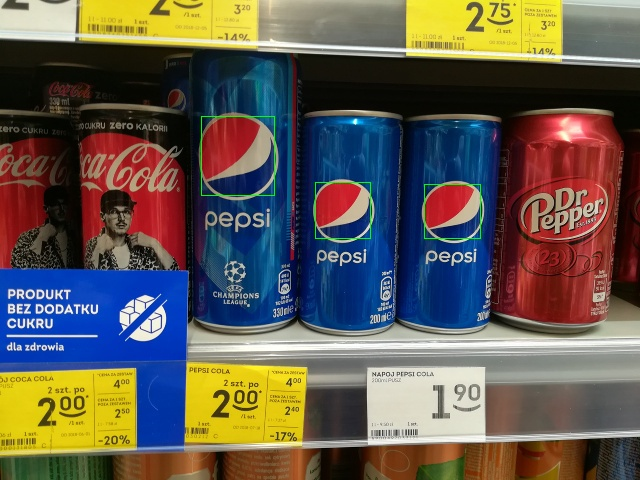
\includegraphics[width=\textwidth]{img/camera/0}
	    \end{subfigure}
	    ~
	    \begin{subfigure}[b]{0.48\textwidth}
	        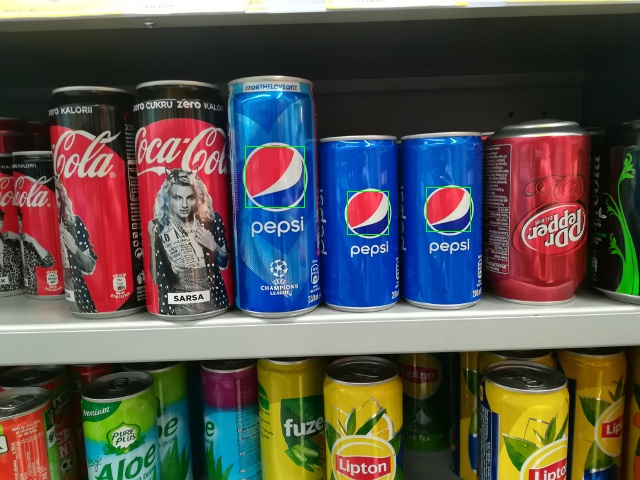
\includegraphics[width=\textwidth]{img/camera/10}
	    \end{subfigure}
	    \\
	    \begin{subfigure}[b]{0.48\textwidth}
	        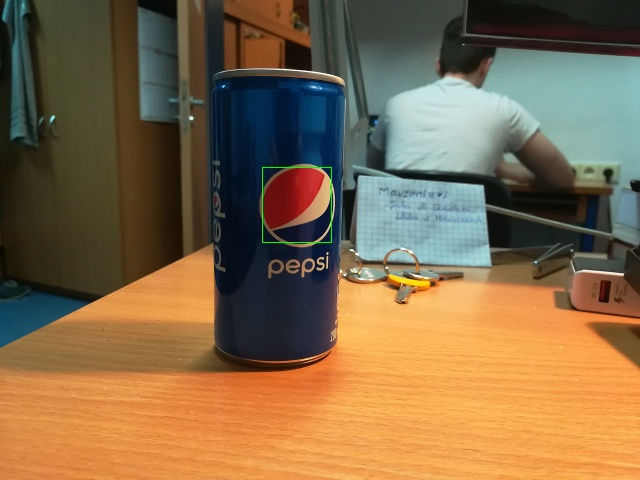
\includegraphics[width=\textwidth]{img/camera/2}
	    \end{subfigure}
	    ~
	    \begin{subfigure}[b]{0.48\textwidth}
	        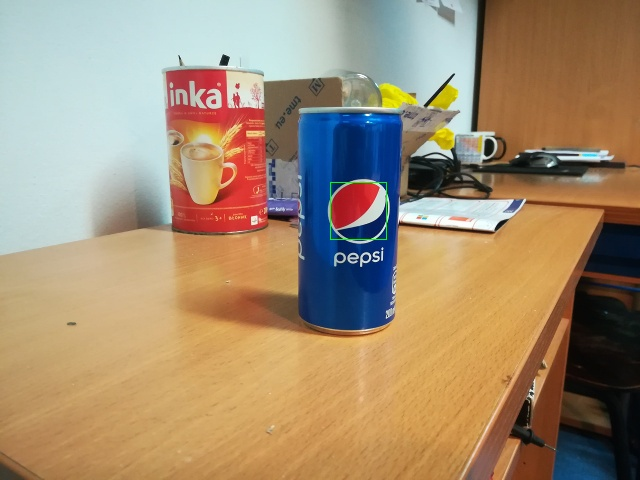
\includegraphics[width=\textwidth]{img/camera/3}
	    \end{subfigure}
	    \begin{subfigure}[b]{0.48\textwidth}
	        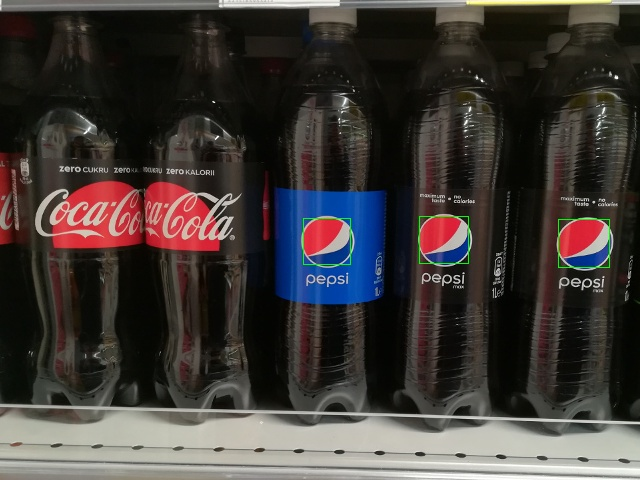
\includegraphics[width=\textwidth]{img/camera/4}
	    \end{subfigure}
	    ~
	    \begin{subfigure}[b]{0.48\textwidth}
	        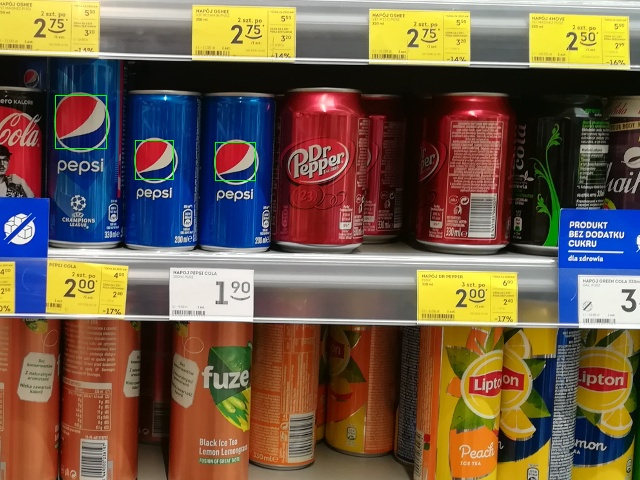
\includegraphics[width=\textwidth]{img/camera/5}
	    \end{subfigure}
	    \begin{subfigure}[b]{0.48\textwidth}
	        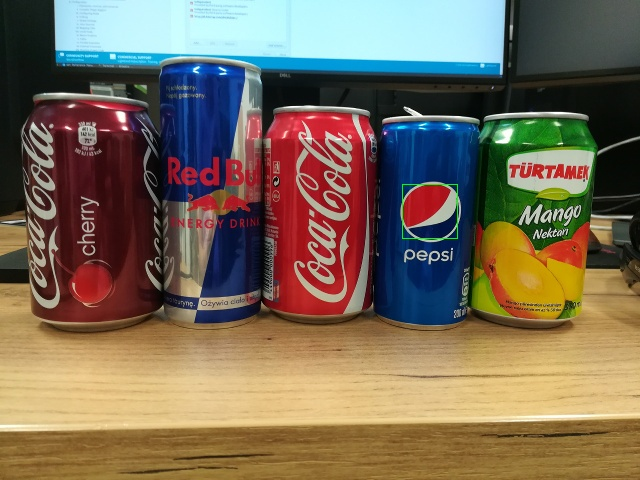
\includegraphics[width=\textwidth]{img/camera/6}
	    \end{subfigure}
	    ~
	    \begin{subfigure}[b]{0.48\textwidth}
	        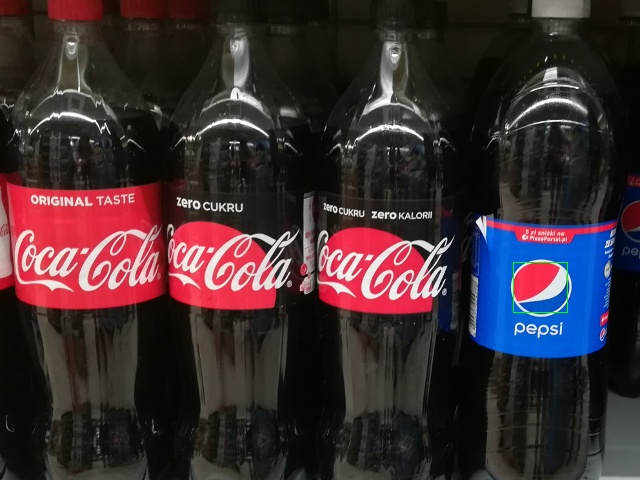
\includegraphics[width=\textwidth]{img/camera/8}
	    \end{subfigure}
	    \caption{Wyniki działania programu dla zdjęć pochodzących ze smartfonu (ciąg dalszy)}
	    \label{fig:smartfon-1}
	\end{figure}

	\begin{figure}
	    \centering
	    \begin{subfigure}[b]{0.48\textwidth}
	        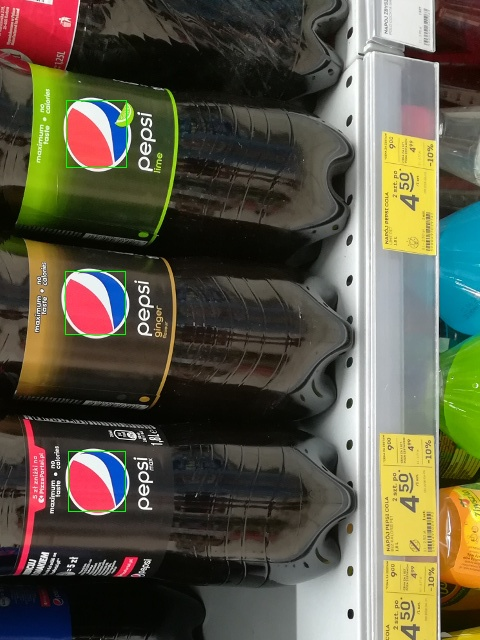
\includegraphics[width=\textwidth]{img/camera/15}
	    \end{subfigure}
	    ~
	    \begin{subfigure}[b]{0.48\textwidth}
	        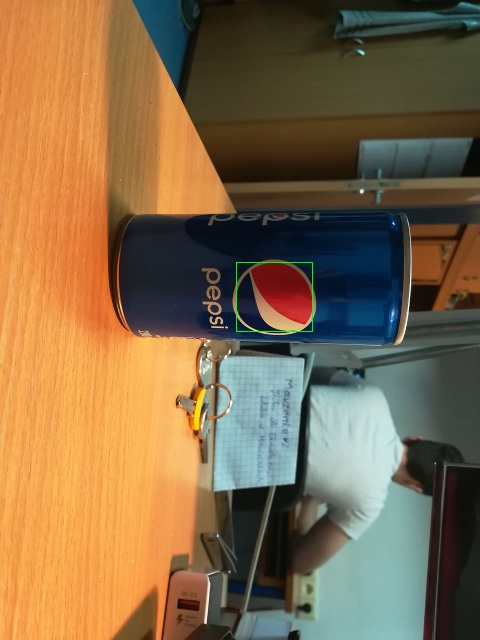
\includegraphics[width=\textwidth]{img/camera/14}
	    \end{subfigure}
	    \\
	    \begin{subfigure}[b]{0.8\textwidth}
	        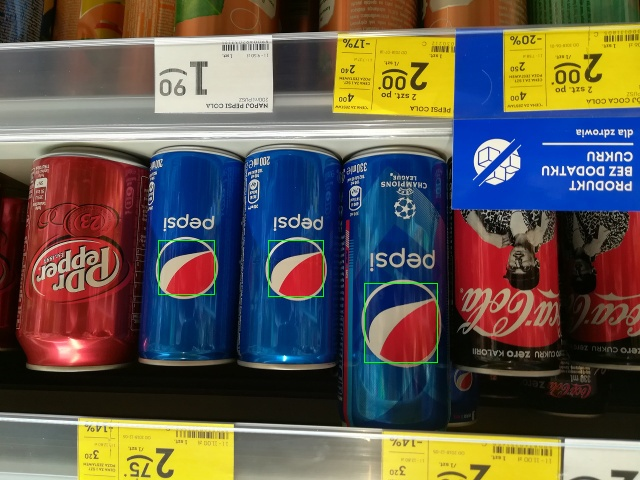
\includegraphics[width=\textwidth]{img/camera/13}
	    \end{subfigure}
	    \caption{Wyniki działania programu dla zdjęć pochodzących ze smartfonu (obrócone zdjęcia)}
	    \label{fig:smartfon-2}
	\end{figure}

	\begin{figure}
	    \centering
	    \begin{subfigure}[b]{0.8\textwidth}
	        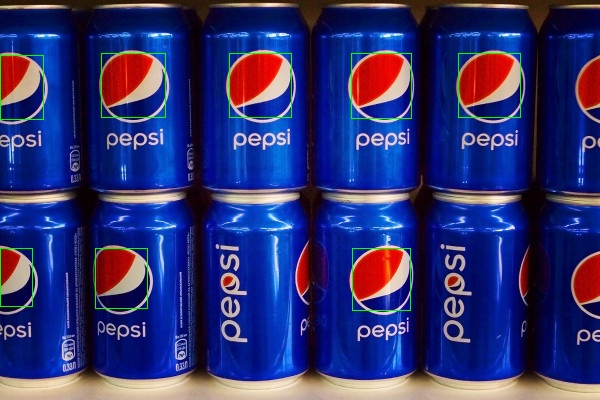
\includegraphics[width=\textwidth]{img/net/0}
	    \end{subfigure}
	    \\
	    \begin{subfigure}[b]{0.8\textwidth}
	        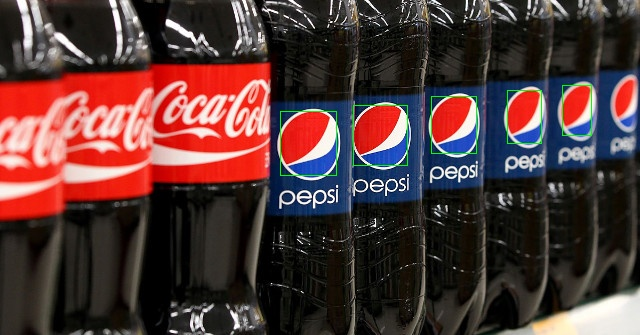
\includegraphics[width=\textwidth]{img/net/1}
	    \end{subfigure}
	    \\
	    \begin{subfigure}[b]{0.8\textwidth}
	        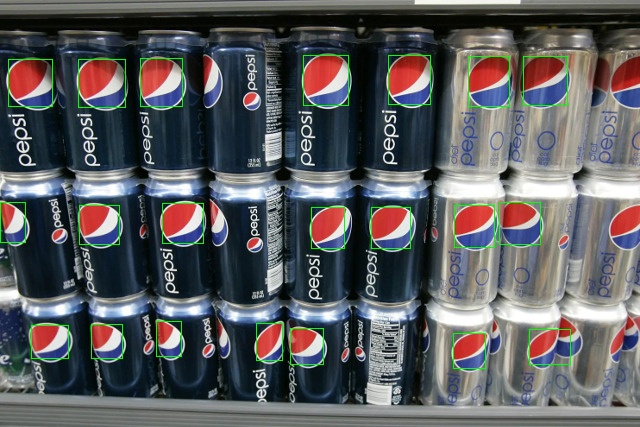
\includegraphics[width=\textwidth]{img/net/2}
	    \end{subfigure}
	    \caption{Wyniki działania programu dla zdjęć pochodzących z internetu}
	    \label{fig:net-1}
	\end{figure}

\section*{6. Zakończenie}

	\subsection*{6.1. Podsumowanie i wnioski}

		Zadaniem projektowym było zaimplementowanie systemu do rozpoznawania loga Pepsi na zdjęciach cyfrowych. Cel ten udało się zrealizować. Zapropowana aplikacja poprawnie rozpoznaje znaczniki na załączonych obrazach. Wraz z aplikacją dostarczono zestaw testów jednostkowych, którymi można zweryfikować poprawność działania algorytmów. Oprócz tego, aplikacja pozwala sprawnie modyfikować parametry działania potoku przetwarzania przy użyciu plików konfiguracyjnych JSON.

		Do oczywistych wniosków należy fakt, iż zaproponowane metody przetwarzania obrazów są silnie zależne od przestrzenii barw i oświetlenia, w jakim robione są zdjęcia. O ile dla zdjęć robionych własną kamerą (gdzie parametry koloru niewiele się zmieniają), nawet dla dynamicznych warunków oświetleniowych, łatwo było znaleźć odpowiednie wartości zakresów progowania. Niestety, dla zdjęć pobranych z internetu, gdzie niemal każde zdjęcie cechuje się inną jakością oraz ilością kolorów, dobranie parametrów algorytmu nie jest zadaniem prostym. Autorzy tych zdjęć często sami je ulepszają oraz wyrównywają poziomy jasności, przez co algorytm staje się bardzo czuły i łatwo generuje błędy już na etapie progowania.

	\subsection*{6.2. Perspektywy rozwoju}

		Jako, że logo Pepsi nie jest skomplikowane, zastosowano stosunkowo proste algorytmy przetwarzania obrazów. Niemniej, rozwiązanie to można dalej rozbudowywać.

		Dalsze ulepszenia potoku przetwarzania dotyczyć mogą przede wszystkim rozpoznawania okręgów z logiem Pepsi. Wykorzystać można w tym celu transformatę Hougha i detekcję krawędzi algorytmem Canny'ego. Dalsze etapy przetwarzania można wtedy ograniczyć tylko do środków okręgów (ponieważ to w nich zawiera się ``centrum'' loga Pepsi). Przynieść to może potencjalnie wzrost wydajności (znacznie mniej pikseli do przetwarzania), jednak należałoby przy tym uwzględnić koszt samej transformaty Hougha.

		Aplikacja została także stworzona z myślą o możliwości rozpoznawania nie tylko loga Pepsi. Do dyspozycji jest interfejs bazowy \texttt{LogoDetector}, zatem należałoby tylko napisać kolejne klasy konkretne, jak np. \texttt{SevenUpLogoDetector}, \texttt{LiptonLogoDetector}, \texttt{SpriteLogoDetector}. Stwarza to potencjalne możliwości rozwoju aplikacji.

\end{document}
